\section{Functional Requirements}
\subsection{Introduction}

\subsubsection{Scope}
The subsystem should be implemented with in the currents AutoMart system and should not replace it. The subsystem needs to provide features that will help AutoMart reduce the number of poor and irrelevant advertisements on their website.

The subsystem is to be implemented in the front end of the system. When the user submits the their advert on the website, the subsystem needs to take the adverts images and evaluate them in order to decide whether the advert wished to be uploaded by the user should be allowed to be entered into the systems database.

The subsystem performs four sequential tests on the adverts images. For each image uploaded a image object will be created and used to store image information. The first test checks if the image uploaded contains a car. If the system detects a car in the image, the test is seen as successful and goes on to the next test. If the system does not detect a car in the image, further image tests come to a halt. A relevant message will be stored in the image object and the system proceeds onto the next image. The second test determines the colour of the car. After the colour has been determined it stores the colour  into the image object. Further testing can proceed even if the system was unable to determine the colour. Third test tries to determine the make of the car. The detected make is stored in the image object and proceeds onto the final test. If the system was unable to detect a make of the car, the testing comes to a halt. Final test tries to determine the model of the car. It uses previous test information to help it determine the model of the car. If the model is determined the information is stored into the image object and proceeds onto the next image.

After all the images have been put through the tests, the image objects representing the images are  put through a final set of tests to ensure that there is no information conflict. The system first checks if all the objects have the same colour. If  there is conflict it tries to resolve it by checking how many object have the same colour and how many don't. The information is also compared against the textual data. If the colour differs between the objects or it differs from the textual data the system will conclude that the images are representing different cars. This would mean that the advertisement is invalid and further testing will halt, and the advert will not be allowed to be uploaded to the system. The second test compares all the make information. If conflict is encountered the same principles as with in the colour conflict will be applied. Finally, the last test compares all the model information. The model testing will be more lenient than the first two tests. If the models differ in most of the objects and also differ from textual data, the textual data will be used to state the model of the car.

After all the test have been passed or halted unexpectedly, the system will provide relevant error messages or informative messages that were encountered during the image testing. The user will have a chance to fix any of the errors a system encountered. If the test were successful  initially or after the user has fixed the errors the advert will be allowed to be uploaded to the system.

Because the system is working with ever changing product, the system needs to accommodate for learning new cars. This way the system will never become unusable at a later stage as it will be able to stay updated with new cars.
\pagebreak
\begin{figure}[h!]
  \caption{High Level System Use Case Diagram.}
  \centering
	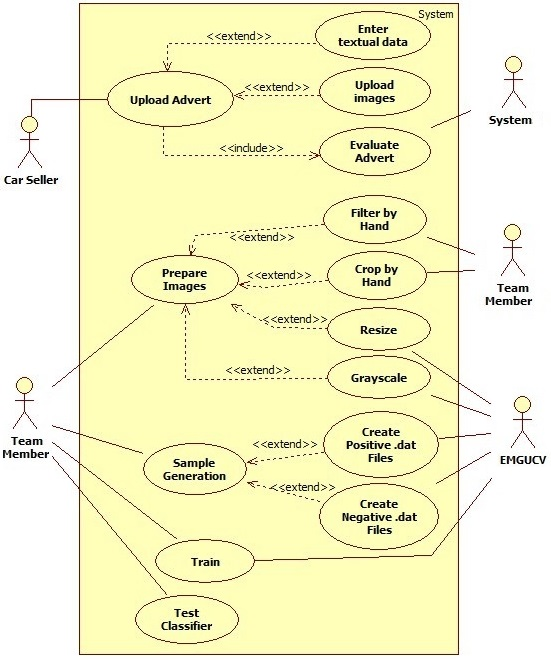
\includegraphics{HighLevelSystemUseCase.jpg}
\end{figure}

\subsubsection{Limitations}
The system may be limited on model recognition, as sometimes it is not possible to distinguish the model of the car by only face value properties that are given by an image. Therefore the system may not be able to determine the model of the car correctly every time.

\subsubsection{Exclusions}
The system should only be implemented to work with cars and should not consider for the existence of any other motor vehicles such as motorcycles and trucks.

\subsection{Required Functionality}
\begin{figure}[h!]
  \caption{Detect Car Low Level Use Case Diagram.}
  \centering
	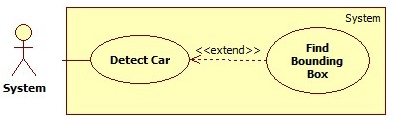
\includegraphics{DetectCarLowLevelUseCaseDiagram.jpg}
\end{figure}

\begin{figure}[h!]
  \caption{Describe Car Low Level Use Case Diagram.}
  \centering
	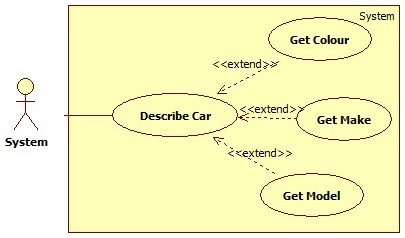
\includegraphics{DescribeCarLowLevelUseCaseDiagram.jpg}
\end{figure}

\begin{figure}[h!]
  \caption{Generate Rating Low Level Use Case Diagram.}
  \centering
	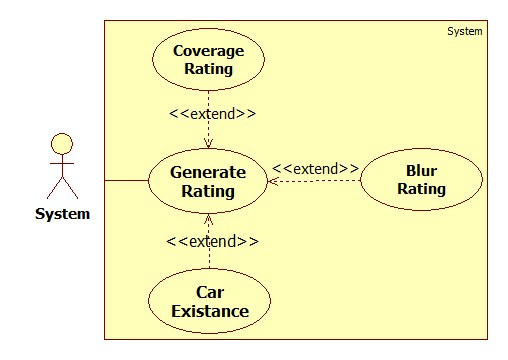
\includegraphics{GenerateRatingLowLevelUseCaseDiagram.jpg}
\end{figure}

\subsection{Use Case Prioritization}
\begin{tabular}{| l | l |}
	\hline
	Use Case & Priority \\
	\hline
	Detect Car & Critical \\
	Find Bounding Box & Important \\
	Describe Car & Critical \\
	Get Colour & Important \\	
	Get Make & Important \\
	Get Model & Nice to Have \\
	Generate Rating & Critical \\
	\hline
\end{tabular}

\subsection{Use Case/Services Contracts}
\textbf{Detect Car} \\
\begin{tabular}{| l | l |}
	\hline
	Pre-Condition & Valid image file. \\
	\hline
	Post-Condition & \\
	\hline
\end{tabular}
\\
\\
\textbf{Find Bounding Box} \\
\begin{tabular}{| l | l |}
	\hline
	Pre-Condition & Trained classifier exists.\\
	\hline
	Post-Condition & \\
	\hline
\end{tabular}
\\
\\
\textbf{Describe Car} \\
\begin{tabular}{| l | l |}
	\hline
	Pre-Condition & A car must exist in the photo.\\
	\hline
	Post-Condition & Car details generated.\\
	\hline
\end{tabular}
\\
\\
\textbf{Get Colour} \\
\begin{tabular}{| l | l |}
	\hline
	Pre-Condition & A car must exist in the photo.\\
	\hline
	Post-Condition & \\
	\hline
\end{tabular}
\\
\\
\textbf{Get Make} \\
\begin{tabular}{| l | l |}
	\hline
	Pre-Condition & Car must be classified.\\
	\hline
	Post-Condition & \\
	\hline
\end{tabular}
\\
\\
\textbf{Get Model} \\
\begin{tabular}{| l | l |}
	\hline
	Pre-Condition & Car must be classified.\\
	\hline
	Post-Condition & \\
	\hline
\end{tabular}
\\
\\
\textbf{Generate Rating}  \\
\begin{tabular}{| l | l |}
	\hline
	Pre-Condition & A car must exist in the photo.\\
	\hline
	Post-Condition & Rating given in range [0, 100].\\
	\hline
\end{tabular}
\\
\\
\subsection{Process Specifications}

\subsection{Domain Objects}
